\PassOptionsToPackage{unicode}{hyperref}
\PassOptionsToPackage{hyphens}{url}
\documentclass[11pt]{article}
\usepackage[margin=1in]{geometry}
\usepackage{xcolor,amsmath,amssymb}
\usepackage{iftex}
\ifPDFTeX
  \usepackage[T1]{fontenc}
  \usepackage[utf8]{inputenc}
\else
  \usepackage{unicode-math}
  \defaultfontfeatures{Scale=MatchLowercase}
  \defaultfontfeatures[\rmfamily]{Ligatures=TeX,Scale=1}
\fi
\usepackage{lmodern}
\usepackage{bookmark}
\usepackage{xurl}
\urlstyle{same}
\usepackage{microtype}
\usepackage{fancyhdr}
\usepackage{longtable,booktabs}
\usepackage{tikz}
\usetikzlibrary{arrows.meta,positioning,calc}
\definecolor{NimbusBlue}{HTML}{233F58}
\definecolor{NimbusLight}{HTML}{EDF3F7}
\AtBeginDocument{\hypersetup{linkcolor=NimbusBlue,filecolor=NimbusBlue,urlcolor=NimbusBlue,citecolor=NimbusBlue}}
\setlength{\emergencystretch}{3em}
\setlength{\parskip}{0.45em}
\setlength{\parindent}{0pt}
\pagestyle{fancy}
\fancyhf{}
\fancyhead[L]{\small\sffamily Nimbus}
\fancyhead[R]{\small\sffamily Technical documentation}
\fancyfoot[C]{\small\thepage}
\renewcommand{\headrulewidth}{0.3pt}
\AtBeginDocument{\setlength{\headheight}{15pt}}
\providecommand{\tightlist}{\setlength{\itemsep}{0pt}\setlength{\parskip}{0pt}}

\hypersetup{pdftitle={Nimbus Studio: Working with simulations and scientific figures},
  pdfauthor={Nimbus project documentation},
  pdfcreator={LaTeX via Tectonic},colorlinks=true}
\title{Nimbus Studio\\\large Working with simulations and scientific figures}
\author{Nimbus project documentation}
\date{18 October 2026}
\begin{document}
\hypersetup{pageanchor=false}
\maketitle
\hypersetup{pageanchor=true}
\pagenumbering{roman}
{\small\setlength{\parskip}{0pt}\setcounter{tocdepth}{2}\tableofcontents}
\clearpage
\pagenumbering{arabic}
\section{What Studio does and where it stops}
Nimbus Studio is the desktop workspace for setting up atmospheric experiments,
launching the Nimbus executable, inspecting saved fields, comparing datasets and
publishing figures. It gives one experiment a common place for its configuration,
run status, data sources, plots and analysis recipes. The intent is to make careful
experimentation practical on ordinary computers without requiring each researcher
to rewrite a model or build a separate visualization application.

The atmospheric solver and Studio are independent programs. The solver advances
the equations; Studio displays products the solver has published. A camera move,
color change or Python analysis does not advance or modify the simulated state.
Closing a plot does not delete the simulation's output. Conversely, a pleasing
render is not evidence that its source experiment satisfies a conservation,
convergence or scientific-validation requirement.

Nimbus was independently developed from the beginning. CM1 appears in Studio as a
read-only dataset and configuration-interchange source, not as the engine behind
Nimbus. Similar variable names or familiar controls do not imply identical
equations, initial conditions, closures or numerics. Use the
\href{MATHEMATICS.pdf}{mathematics guide} for those assumptions and the
\href{ARCHITECTURE.pdf}{architecture guide} for solver ownership and execution.

This guide follows the ordinary application paths. It describes implemented
features and their admission checks, including intentionally unavailable paths.
It does not certify every machine, renderer, field combination or scientific
interpretation. The terms Ready and Fully Qualified retain the repository's
meaning: bounded tests, completed long campaigns and independent scientific
review are distinct evidence. A successful image is only one part of that chain.

\begin{figure}[htbp]
\centering
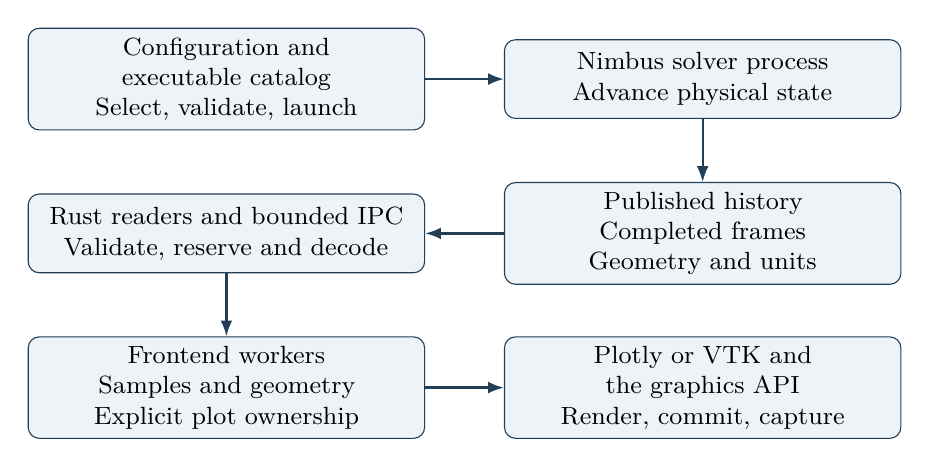
\begin{tikzpicture}[
  box/.style={draw=NimbusBlue,rounded corners,fill=NimbusLight,align=center,
    text width=4.8cm,minimum height=1.0cm,font=\small},
  flow/.style={-{Latex[length=2mm]},thick,draw=NimbusBlue}]
\node[box] (config) {Configuration and executable catalog\\Select, validate, launch};
\node[box,right=1.0cm of config] (solver) {Nimbus solver process\\Advance physical state};
\node[box,below=0.8cm of solver] (history) {Published history\\Completed frames\\Geometry and units};
\node[box,left=1.0cm of history] (reader) {Rust readers and bounded IPC\\Validate, reserve and decode};
\node[box,below=0.8cm of reader] (worker) {Frontend workers\\Samples and geometry\\Explicit plot ownership};
\node[box,right=1.0cm of worker] (screen) {Plotly or VTK and the graphics API\\Render, commit, capture};
\draw[flow] (config) -- (solver);
\draw[flow] (solver) -- (history);
\draw[flow] (history) -- (reader);
\draw[flow] (reader) -- (worker);
\draw[flow] (worker) -- (screen);
\end{tikzpicture}
\caption{The solver publishes data across a process boundary. Studio renders
those data through a separate ownership chain. Imported histories enter at the
reader boundary; changing the view does not feed back into the solver.}
\end{figure}


\subsection{The first launch has no storm to display}
A fresh checkout and fresh Studio profile contain no pre-run simulations. The
Runs view may be empty; the Plots workspace offers \textbf{Open data}. These are
normal states. Studio can open, show configuration controls and report its
preferences without running the solver or downloading scientific runtime tables.
The \href{BUILDING.md}{build guide} describes a build-and-open-only check for
Windows, Linux and macOS. This is the appropriate first check on a new machine.

There are then two ordinary ways to obtain a dataset. Open an existing Nimbus
run or supported CM1 history through Open data, or configure and launch a Nimbus
experiment. A run directory is the useful unit of Nimbus data: its metadata and
completion records give meaning to the field files. Selecting an arbitrary array
without that context cannot reconstruct its coordinate system, units, valid
domain or simulation time.

The native desktop application provides filesystem access, process launch and
native readers. The development browser frontend can exercise rendering and
synthetic harnesses, but its mocked native operations are not a replacement for
the installed application. Browser rendering evidence and native application
evidence should be reported separately.

\subsection{The main working areas}
\textbf{Configure} holds the experiment draft and its launch controls.
\textbf{Runs} exposes launched or discovered histories, status and logs.
\textbf{Plots} opens a data source and builds a viewing workspace. Settings
contains local paths, appearance, loading performance and remote connections.
Projects and investigation workspaces retain related source and view choices so
the user can return to an analysis without treating one transient screen as the
whole experiment.

Preferences such as text size, light or dark appearance and which side holds the
plot affect the desktop workspace. They are not solver configuration. Similarly,
the Loading workers preference controls Studio's field-loading concurrency,
whereas the solver's threading and compute-backend settings belong to the run.
Keep these two kinds of tuning separate when diagnosing performance.

Saved preferences and recent-dataset entries are conveniences, not archives of
the underlying data. Moving or deleting a source can make a saved project
unresolvable. Preserve the source history, configuration and any external inputs
alongside a project when reproducibility matters. Exported investigation and
research packages add explicit recipes and provenance; they do not silently turn
every linked source into an embedded simulation archive.

\section{Configuration, launch and data discovery}
\subsection{A draft must agree with the executable}
The configuration editor combines a structured form with YAML. Public templates
provide starting experiments; they are not certificates for a storm, a resolution
or an arbitrary set of physics choices. The
\href{NAMELIST.md}{complete namelist reference} inventories strict-v1 settings,
omission defaults, units, aliases and restrictions, including options not exposed
as form controls and legacy-reader compatibility.

Studio obtains a scheme catalog from the selected Nimbus executable. The catalog
describes its selectors and admission constraints. A UI label alone does not
establish that the executable implements the requested combination. Validation
and preflight check the actual draft, target, executable identity, required
inputs and configuration dependencies before launch. A configuration can contain
individually recognizable schemes while their coupling is still rejected.

Scientific tables are separate runtime inputs. Thompson and RRTMG requirements
are described in the build guide; opening Studio does not imply that these
tables have been installed. Provisioning a canonical table set and checking its
identity prevents compiler-dependent reconstruction from silently substituting
different input bytes. A missing input should be repaired at its reported path,
not bypassed by changing an unrelated numerical tolerance.

The binary-path preference selects an executable when automatic discovery is
not the intended build. The runs-directory preference selects the library root
for newly launched histories. Inspect these settings when several checkouts or
installed versions coexist: the source tree being edited and the executable
being launched are not necessarily the same build.

\subsection{Run status and continuation}
Launching creates a separate solver process. Studio collects status and log
information; run progress and saved-frame availability are different signals.
A process may be advancing while no new output frame is complete. Conversely,
a finished process can leave useful completed frames even when a later operation
failed. Read the reported outcome and logs rather than interpreting the presence
of a directory as success.

Checkpoint inspection belongs to continuation, not to plotting. A history frame
contains display products; a valid continuation must retain all state required
by the selected runtime. Do not assume that being able to plot a time means it
is a restart endpoint. The executable's checkpoint and configuration checks
remain authoritative when preparing a continuation.

\subsection{Nimbus histories and imported histories}
Nimbus output readers support the maintained NPY, ZFP and netCDF history paths.
NPY remains supported while the required netCDF replacement scope is being
completed and qualified. ZFP is a storage codec, not a new coordinate system or
a guarantee of losslessness: retain the output's compression provenance when
comparing values. Opening a compressed field should not erase how its values
were encoded.

A published output hierarchy can provide checksummed levels of detail and
bounded native reads. Without such a hierarchy, level zero still has its native
read contract; Studio must not invent a published coarse product merely because
it can produce a smaller display. Source selection records whether a plot uses
a published level, a bounded source window, a reduction or display reconstruction.

CM1 import can inspect history files, a case directory, namelist information and
an input sounding. Its compatibility and decision views distinguish direct
mechanical mappings from unresolved scientific decisions. Translation can produce
a partial draft that still needs interpretation. Nimbus does not install or run
CM1, and importing CM1 data does not make Nimbus a CM1 fork.

An adapter records source kind, locator, geometry and availability. Rank matters:
a two-dimensional column product cannot enable a three-dimensional renderer just
because its field name looks atmospheric. Vector views also require physically
matched components. The plot picker therefore uses dataset capabilities rather
than presenting every plot as if every file could satisfy it.

\subsection{Health and alignment are part of opening data}
Dataset health checks expose missing fields, shape or coordinate disagreements,
time-axis problems and incomplete products. Treat a missing value as missing,
not as calm wind, dry air or zero precipitation. A finite array value is not by
itself proof that the location lies inside the physical domain: halos and boundary
closure planes are excluded according to the saved geometry.

For comparisons, inspect the alignment report before interpreting a difference.
Time, physical coordinates, units, component meaning and valid-domain support
must match the requested operation. A common shape is insufficient: two arrays
can have equal dimensions but different origins, spacings, model frames or units.
When an operation requires aligned grids, a rejected mismatch is useful feedback,
not a reason to strip the metadata.

\subsection{A practical first inspection}
Open a completed history and start with one scalar Slice. Check its field name,
units, saved time, axis labels, slice location and source disclosure. Move to a
second completed frame and confirm that both the values and time label change.
Then add a vertical profile or cross section through an identifiable feature.
Only after those coordinate checks should a volume or composite storm scene be
used to explain the feature's three-dimensional appearance.

This sequence makes a dense 3-D view easier to interpret. An opaque volume can
hide an interior maximum; a threshold surface omits everything below its chosen
level; a derived diagnostic can require fields that were never exported. A simple
slice provides a direct way to distinguish a data problem from a camera,
transfer-function or feature-selection problem.

\section{Reading a plot as a scientific statement}
\subsection{Coordinates come before color}
A field is more than a rectangular array. It has a location on a grid, a physical
unit, a domain mask and a saved time. A C-grid velocity component lives on its
own faces; a scalar often lives at cell centers. Earth-frame winds, model-frame
winds and terrain-normal transport components cannot be exchanged solely because
all three have velocity units. Studio's coordinate and vector helpers preserve
these distinctions or reject a view that lacks the required geometry.

Cartesian axes can be translated or nonuniform. Terrain-following levels can
have different physical heights in each column. Cylindrical geometry includes
an angular coordinate. If physical coordinates are unavailable, the application
must identify index units rather than attach metres to an index. The source's
physical-domain bounds determine what may be drawn and reduced; allocated halos
do not become extra atmosphere.

The first two slice indices identify the horizontal directions and the third
identifies the vertical direction in the normalized field representation. A
plan view holds the vertical index fixed. A vertical section holds a horizontal
index fixed. The displayed axes and coordinate metadata, rather than an old
internal variable name, establish whether an axis means Cartesian distance,
angle, height or model level. The plot labelled \textbf{X profile}, for example,
is a Cartesian profile along $x$ at fixed $y$ and $z$; the historical component
filename does not make it a radial average.

\subsection{Slice, vector and composite views}
\textbf{Slice} draws a scalar plane. Changing the slice index requests the
corresponding plane; zoom changes the viewport. For window-capable sources these
operations can request a bounded portion of the source rather than load the
entire three-dimensional field. The source shape, window origin, extent, stride
and aggregation explain what was returned. A lower-resolution display must not
be reported as native merely because its pixels fill the window.

For terrain data, a horizontal model-level plane remains a model-level view:
its height can vary horizontally. The vertical-slice path remaps its one-cell
thick bounded window onto separable physical coordinates before Plotly displays
it. This makes height meaningful on the vertical axis, but it is a documented
remapping operation, not an assertion that the original terrain grid was flat.
Retain the corresponding disclosure when exporting or comparing the view.

\textbf{Vector field} draws arrows for a physically matched component family.
The in-plane components depend on the selected section. Arrow density and scale
affect readability; reducing arrow count does not filter the underlying velocity
field into a new scientific result. Check the frame convention and units before
interpreting arrow direction as Earth-relative motion. A section cannot borrow
an unrelated component solely to make a third arrow coordinate available.

\textbf{Composite} combines a filled scalar plane with contour overlays and
available vector context. Each layer must refer to the same admitted source
plane and frame. Contour thresholds state an explicit condition on values; color
and line width are display choices. If a required overlay is absent or still
loading, a composite cannot truthfully claim that all selected layers have
finished. An older completed view may be retained while its replacement is
prepared, with completion and capture bound to the actual displayed identity.

Deselecting the active field is a valid empty state. It should produce a clear
\emph{No data to plot} state and release unused requests, rather than accuse the
run of failing to export a field the user no longer requested. This distinction
also matters to error handling: an empty selection, a pending read and a genuine
missing export are different conditions.

\subsection{Zoom, native cells and smooth display}
A screen has a finite pixel count; a dataset can have many more cells. Studio
therefore separates the source samples, samples admitted for a particular view,
and the raster used to draw that view. Zooming can refine a bounded preview, but
it cannot recover structures absent from the source. A blocky native-cell plot
at extreme zoom is sometimes an honest view of the model's resolution.

Plotly's heatmap smoothing control changes shading only. It is applied to
regular, finite heatmaps with suitable linear axes. Nonuniform coordinates,
missing values, unsuitable axes and incompatible array shapes retain the
original shading. In particular, smoothing must not bridge a missing-data hole
or reinterpret a stretched coordinate as uniform. The control discloses when
original shading is retained.

For two neighbouring finite samples, linear interpolation has the form
\begin{equation}
 q(\xi)=(1-\xi)q_0+\xi q_1,\qquad 0\leq\xi\leq1.
\end{equation}
This interpolant is bounded by those samples. It can make their transition look
smooth but contributes no new independent measurement between them. Two- and
three-dimensional linear reconstruction apply the corresponding tensor-product
weights. Smoothing a threshold surface is a different operation and belongs to
the disclosed presentation mode described below.

The canvas also follows display pixel density so labels and graphical elements
remain legible on high-density screens. That adjustment is independent of the
simulation's cell spacing. A higher-resolution PNG can improve text and edge
appearance; it cannot turn a coarse numerical field into a fine-grid result.
For publication, preserve units, color limits and sampling disclosure alongside
the image rather than treating pixel count as a scientific resolution measure.

\subsection{Profiles, soundings and hodographs}
\textbf{Vertical} displays a scalar against height at a selected column.
\textbf{X profile} displays a scalar along the Cartesian $x$ direction at fixed
$y$ and $z$. Missing support creates gaps rather than a fabricated continuous
line. Check whether the vertical coordinate is physical height or a declared
model-level coordinate; a level number is not an altitude.

\textbf{Hodograph} plots $u(z)$ against $v(z)$. Its two horizontal axes must use
compatible velocity units and equal geometric scale for direction and turning
to remain interpretable. Height is the parameter along the curve, not a third
horizontal wind component. Storm-relative analysis requires an explicit motion
estimate; translating a hodograph changes its reference frame, not the saved
Earth-relative wind.

\textbf{Skew-T} uses a skewed temperature coordinate and logarithmic pressure
representation. Pressure and either temperature or potential temperature are
required; additional thermodynamic curves require their corresponding inputs.
Do not interpret a missing moisture curve as zero humidity. Sounding plots use
a portrait-friendly layout because forcing the diagram into a very wide, short
pane distorts the geometry that readers use to judge its slopes.

The plotted environmental profile and a parcel-theory interpretation are also
different objects. A sounding's appearance alone does not establish CAPE, parcel
origin, entrainment assumptions or a storm's future development. Retain those
assumptions in the analysis or script used to derive a diagnostic.

\subsection{Time series, time-height plots and swaths}
\textbf{Time-series} applies a declared reducer to a field over completed saved
frames. Mean, minimum, maximum and other offered reductions answer different
questions. A native-cell arithmetic mean is not automatically a mass-weighted
or volume-weighted integral, especially on stretched grids. Read the selected
reducer and geometry rather than infer a conservation statement from a smooth
curve. The horizontal coordinate is saved simulation time, not the wall-clock
time required to load the frame.

\textbf{Time-height} retains a vertical level while reducing the other
directions, producing a Hovmöller-style diagram. Irregular output times and
physical height coordinates must remain visible in its geometry. Large gaps
between saved frames are not observations of what happened between them.
Height-bin averaging and native model-level reduction should not be confused.

\textbf{Swath} accumulates a selected per-cell maximum or minimum across saved
frames. This is a history product: an intense swath location need not correspond
to the currently selected frame. Moving-domain data require explicit Earth-frame
placement if the intended result is a geographic storm track. A moving grid's
array index does not stay over the same Earth location. The swath implementation
tracks source motion where the necessary metadata are available.

These views can read many frames. Their cost may therefore be dominated by
storage and reductions rather than graphics. Changing the requested history
range or field should cancel obsolete work, while shared useful reads may stay
active for other consumers. An analysis assembled from fewer saved frames has
less temporal information even if its display interpolates smoothly.

\subsection{Radar products}
The Radar category uses product presets rather than a separate universal radar
solver. It selects supported reflectivity-related views from the available
dataset. A simulated reflectivity diagnostic is not itself an observed radar
scan, and a color scale does not supply beam geometry or observational effects
that the diagnostic did not calculate.

Logarithmic reflectivity requires care when reducing it. Averaging decibels and
averaging linear reflectivity are different operations. For values $D_i$ in dBZ,
a linear-reflectivity mean is
\begin{equation}
 \overline D=10\log_{10}\!\left(\frac{1}{n}
       \sum_{i=1}^{n}10^{D_i/10}\right).
\end{equation}
The sampling disclosure distinguishes a bounded linear-$Z$ mean from ordinary
cell means and extrema. A radar floor in a three-dimensional view is an
additional layer with its own source, reduction and color mapping; it must
belong to the same displayed frame as the volume above it.

\section{Three-dimensional views}
\subsection{Scientific mode and presentation mode}
Three-dimensional views distinguish \textbf{scientific} and
\textbf{presentation} fidelity. Scientific mode uses resolved source data with
declared sampling, interpolation and feature extraction. It does not mean that
every source cell is always resident or every pixel is an exact source sample.
Bounded subsampling, cell means, extrema reductions and linear reconstruction
have distinct provenance because they change what one can infer about peaks.

Presentation mode can add explicitly disclosed surface smoothing or
support-constrained subgrid detail. These operations can help explain a scene's
shape and continuity. They do not establish new resolved vortices, cloud scales
or physical gradients. Changing fidelity is separate from choosing graphics
quality, ray-step density or screen resolution. A lower-cost scientific render
can still be scientifically honest when its reduction is accurately reported.

Sampling provenance records the source lattice, retained lattice and display
lattice independently. It also records coordinate resampling, including
linear-to-uniform resampling of stretched axes or physical-volume terrain
remapping. In a multi-layer scene, the overall disclosure must account for its
coarsest contributing sampling; a native-resolution foreground cannot make a
coarse background native.

\subsection{Volume rendering}
\textbf{Volume} displays a three-dimensional scalar through a color transfer
function and an opacity transfer function. Color answers what value was sampled;
opacity determines how strongly it contributes along the viewing ray. A bright
or solid-looking region is therefore a consequence of both the field and the
chosen transfer function. Different camera directions can expose or hide the
same interior structure without changing the source.

The renderer samples a ray through a bounded volume texture, respecting validity
support and the scene's coordinate transform. Missing cells should not become
opaque zero-valued material. Interpolating near missing support needs validity
handling, not just a color for NaN. Texture capacity and rendering budgets can
require a bounded representation; source disclosure remains attached to it.

Color range, opacity range and any threshold answer different questions. Fixing
a color range across frames makes visual comparison easier; recomputing a range
for each frame can reveal weak structure but can also make unchanged colors
represent different values. Read the colorbar and range policy when interpreting
growth or decay. Outlier-resistant display ranges can improve visibility while
leaving extrema outside the emphasized range; they do not redefine those extrema.

\subsection{Isosurfaces}
\textbf{Isosurface} extracts the set where a scalar crosses a chosen threshold,
using a marching-cubes family of extraction paths. A threshold surface is a
geometric representation of a level set, not a material boundary unless the
scientific interpretation justifies that identification. Its shape depends on
the threshold, source sampling, interpolation and any declared smoothing.

The preparation pipeline can keep scalar backing and extracted geometry in
workers for reuse. Reusing a previous contour is valid only when the current
prepared dataset identity matches the backing that produced it. Equal field
names, equal dimensions or an apparently familiar frame do not prove that a
worker still holds the same bytes. When a source is evicted and prepared again,
its new resident identity forces the appropriate rebuild.

Lighting changes should not require rebuilding the level set. They update its
material and then the committed appearance descriptor, preserving the source
and geometry identity. The capture metadata must describe the lighting actually
drawn. An export containing the new pixels with the old shadow or fill settings
would be an inconsistent scientific figure recipe.

\subsection{Streamlines and parcel paths}
\textbf{Streamlines} integrate through a vector field at one saved time. The
seed region, direction, integration limits and available support determine the
curves. A streamline is tangent to the instantaneous vector field; it is not
automatically the trajectory of an air parcel through a time-varying storm.
Velocity and vorticity streamline choices require the corresponding coherent
vector field and valid coordinate interpretation.

Geometry preparation, vector sampling and seed selection are distinct from
tube width, color and lighting. A thinner line is not a weaker wind. Cropping
the seed region can reveal the requested feature and reduce work, but omitted
seeds do not establish that other flow paths do not exist. Invalid or unsupported
locations terminate or exclude integration according to the extraction contract.

\textbf{3D paths} reads saved Lagrangian trajectory products. It therefore needs
trajectory output, not merely a set of instantaneous wind fields. The companion
\textbf{Vorticity budget} view uses the saved parcel tendency terms. These are
history-dependent products and are not per-frame volume renderers. Missing
trajectory export should disable the feature clearly rather than silently
substitute a streamline.

\subsection{Rendered supercell and coordinated layers}
\textbf{Rendered supercell} combines condensate volume with available layers
such as a reflectivity floor, updraft structure and other offered diagnostics.
Its availability starts with a supported cloud or total-condensate field;
optional layers have their own input requirements. This is a composite
visualization, not an additional microphysics scheme or a reconstruction of
unexported fields.

Shared volume composition coordinates geometry, textures and shader evaluation
across participating layers. Overlapping volumes must use consistent domain
transforms and physical sampling. Independently drawing translucent actors in
an arbitrary order can change the image; the composition path therefore owns
their joint ordering and framebuffer use. Nested outputs additionally need
parent/child spatial ownership so overlapping refinement regions are not counted
twice as visual material.

Optional cloud presentation detail and motion cues are declared display
operations. They must remain supported by the source cloud and its coordinate
frame. A moving presentation is not a newly integrated cloud field. Use
scientific mode and a direct slice when a conclusion depends on whether a
small structure actually exists in the exported model samples.

\subsection{Camera, orientation and appearance controls}
The camera has a position, target and orientation relative to the physical
scene. The compass, domain box, axes and elevation controls help make this
relationship explicit. Physical elevation controls need the loaded grid; a
placeholder range before geometry is available must not be interpreted as a
valid model height.

Color, background, light direction, shadow depth, fill tint and material
properties control appearance. They can improve shape perception but also
emphasize features for purely optical reasons. Record them when comparing
images. In particular, a new lighting setting must update the appearance
receipt after a successful redraw without falsely changing the scientific
frame or geometry that the scene contains.

Shared and independent control scopes allow several panes to coordinate some
choices while retaining their own views. Camera synchronization does not prove
that two datasets align scientifically. Confirm source time, domain, units and
sampling before using synchronized views as a comparison.

\section{How a saved field becomes a screen image}
\subsection{Native reading and the process boundary}
React and TypeScript own interaction, view state and rendering preparation.
Tauri's Rust layer owns native filesystem access, readers and process operations.
Large numeric payloads cross the native interface as binary arrays with explicit
metadata rather than as enormous JSON lists. The reader validates dimensions,
types, bounds and source identities before the frontend treats the payload as a
field.

A bounded-window request describes an origin, extent and sampling policy.
Returned bytes and source work are separate quantities. A block mean can return
one value while visiting many source cells; a compressed representation can need
codec scratch in addition to its decoded output. Accounting only for the final
array would underestimate the temporary native read footprint.

The native netCDF API is loaded once and retained for the process lifetime,
while individual file handles are still closed after their operations. This
distinguishes the lifetime of a library's executable code and internal cleanup
state from the lifetime of a dataset file. Repeatedly unloading a library that
has registered process or thread cleanup callbacks can leave callbacks referring
to unloaded code. Keeping the library available does not mean retaining every
opened dataset or bypassing the reader's serialization and memory controls.

\subsection{Workers prepare data without owning the interface}
Web workers perform expensive preparation, derived-field work, contour
extraction, streamline integration and other bounded tasks outside the UI thread.
The interface can remain responsive while a worker scans a field or builds a
mesh. Moving work to a worker does not make it free: memory, transfers, queues
and completion synchronization still contribute to latency.

Array buffers can be transferred between owners rather than repeatedly copied.
A transfer changes who may use the buffer; the sender cannot continue treating a
detached buffer as its live backing. Worker dataset registries therefore record
identity and lifetime, not just a pointer or field label. Geometry caches and
scalar caches have to agree on the actual resident dataset used by a task.

Changing a field or frame creates a new request generation. A completed old task
may no longer be useful when it returns. The result is validated against the
current owner before publication, so late work cannot overwrite the newly
selected view. Cancellation also retires obsolete resource claims. A cache may
retain a deliberately reusable result, but that retention must have an owner and
be represented in the relevant accounting.

\subsection{Plotly and VTK have different jobs}
Plotly handles most two-dimensional figures, profiles, sounding diagrams,
history plots, Python numeric previews and research panels. Its canvas and vector
elements manage axes, labels, selection and zoom. VTK handles the primary
volumetric, surface, streamline and trajectory scenes. It consumes prepared
datasets and geometry, constructs actors and mappers, and submits graphics work
through the chosen browser graphics API.

These are application-rendering paths. The solver's Vulkan and Metal compute
backends do not determine Studio's graphics API. A CPU simulation can be viewed
with GPU rendering; a GPU simulation can be viewed on another computer. The
desktop webview, driver, graphics capability and workload determine which
rendering paths are available.

Volume workloads currently use the WebGL GPU path because the maintained
vtk.js WebGPU volume implementation does not provide the same required shading,
opacity-normal, scattering and close-camera behavior. Geometry workloads can
select WebGPU when adapter discovery and the actual VTK device/context
initialization succeed. A preference alone is not proof that the requested API
became active. Device or initialization failure is disclosed and uses the
maintained WebGL path where available. This rendering fallback is separate from
the solver's native-required compute admission contract.

\subsection{Textures, triangles and shaders}
For a surface or streamline, the CPU or worker prepares vertices and connectivity.
The graphics API uploads geometry, transforms vertices through the scene and
camera matrices, rasterizes primitives and shades their covered pixels. Surface
normals and light directions affect brightness. A bright face can be facing a
light rather than carrying a larger field value; the colorbar describes the
scalar mapping, not the lighting multiplier.

For a volume, a shader samples one or more scalar textures along each viewing
ray. Each sample is mapped to a color and opacity. A simplified front-to-back
composition illustrates the ownership of those choices:
\begin{align}
 C_{j+1} &= C_j+(1-A_j)\alpha_j c_j,\\
 A_{j+1} &= A_j+(1-A_j)\alpha_j.
\end{align}
Here $c_j$ is a sample color, $\alpha_j$ its opacity over the current sample
segment, and $C_j,A_j$ the accumulated color and opacity. Both the step length
and transfer function matter. A physically scaled opacity convention can be
expressed as $\alpha=1-\exp(-\sigma\,\Delta s)$ for an effective attenuation
$\sigma$ and path increment $\Delta s$. This explains why changing sampling
distance without correcting opacity can change how thick a cloud appears.
It is an explanation of rendering, not a replacement for the solver's
radiation calculation.

Texture interpolation, scalar validity, lighting, shadow sampling, background
composition and output color are separate shader responsibilities. Shadows help
depth perception but do not represent the atmospheric heating computed by a
radiation scheme. A reflectivity floor is composited with its own color encoding
and physical plane. The final framebuffer holds rendered pixels; the native
field and its scientific units remain separate data.

\subsection{Context loss and scene reconstruction}
Graphics contexts can be lost because of driver resets, resource pressure or
the browser's management of graphics resources. Once a context is lost, its
old textures and framebuffer attachments cannot be assumed usable. Studio's
owned render-window construction installs traversal protection and framebuffer
ownership together before the VTK object is frozen. Independent patches must
not overwrite one another's guards.

The loss path stops invalid traversal; restoration reconstructs the scene through
its owners. A restored canvas must reach a completed render before it is reported
as a current frame or captured. Merely receiving a context-restored event is not
enough. This boundary prevents a stale texture, half-rebuilt layer or previous
frame's legend from masquerading as the selected result.

Recovery cannot guarantee that every driver or device can support the requested
scene. Persistent failure should remain visible and can require a smaller scene,
different graphics preference or application restart. What the implementation
must preserve is honest state: it cannot silently label invalid or incomplete
pixels as a completed scientific view.

\section{Frame identity, playback and coherent presentation}
\subsection{Requested, loaded and displayed are distinct}
Selecting a saved frame starts a request; it does not immediately replace the
pixels. A field can finish reading before its geometry is prepared, and a scene
can finish preparation before the graphics API draws it. Studio tracks these
stages independently. The displayed time should describe the pixels currently
visible, with the requested frame shown separately when it differs.

Frame identity includes both the saved step and its publication generation.
Reopening a reused directory can produce another run with the same step number.
Matching only that number would accept data from the wrong publication. Multi-
field plots require every contributing array to agree on the exact publication,
not just on shape or step ordinal.

The capture predicate is therefore conceptually
\begin{equation}
 \text{capture allowed} =
 (\text{displayed identity}=\text{requested identity})
 \ \land\ (\text{render complete}).
\end{equation}
The implementation additionally guards the active source and operation while
capture proceeds. A late change in field, view, source or frame invalidates work
that no longer describes the current request.

\begin{figure}[htbp]
\centering
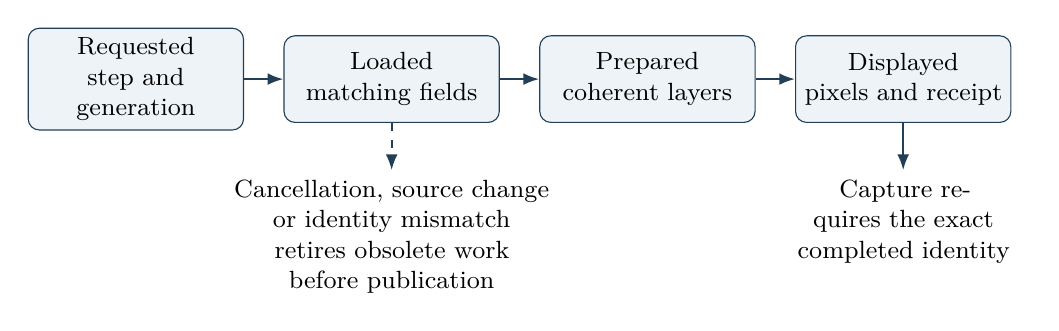
\begin{tikzpicture}[
  box/.style={draw=NimbusBlue,rounded corners,fill=NimbusLight,align=center,
    text width=2.5cm,minimum height=1.1cm,font=\small},
  flow/.style={-{Latex[length=2mm]},thick,draw=NimbusBlue}]
\node[box] (request) {Requested\\step and generation};
\node[box,right=0.5cm of request] (load) {Loaded\\matching fields};
\node[box,right=0.5cm of load] (prepare) {Prepared\\coherent layers};
\node[box,right=0.5cm of prepare] (display) {Displayed\\pixels and receipt};
\draw[flow] (request) -- (load);
\draw[flow] (load) -- (prepare);
\draw[flow] (prepare) -- (display);
\node[below=0.6cm of load,align=center,font=\small,text width=5.4cm] (reject)
  {Cancellation, source change or identity mismatch\\retires obsolete work before publication};
\draw[flow,dashed] (load.south) -- (reject.north);
\node[below=0.6cm of display,align=center,font=\small,text width=3.0cm] (capture)
  {Capture requires the exact\\completed identity};
\draw[flow] (display) -- (capture);
\end{tikzpicture}
\caption{A request is not a displayed frame. The last completed scene may remain
visible during preparation; its label and capture state must continue to describe
that scene until the new one commits.}
\end{figure}


\subsection{Multi-layer scenes commit together}
A cloud volume, updraft surface and radar floor can have different preparation
costs. Publishing each as soon as it happens to finish could mix atmospheric
times in one picture. A coordinated scene keeps the selected generation and
layer identities until the required work is complete. Legends, source disclosure
and capture metadata are committed with the scene they describe.

Appearance-only updates have a smaller boundary: they retain the scientific
frame and geometry, redraw the changed material, then refresh the appearance
part of the capture descriptor. Updating a shadow control must not accidentally
claim that a new scientific field was loaded. Conversely, retaining the right
frame is not permission to leave the recorded lighting recipe stale.

\subsection{Playback is an output-viewing schedule}
Playback advances through saved frames, waiting for the participating views'
required completion contracts. The requested rate is a target; achievable
cadence depends on source I/O, decoding, preparation and rendering. A 60 fps
request does not create model states between saved outputs and does not promise
60 newly rendered scientific frames per second on every machine.

Prefetch can prepare future reads while the current frame is displayed. It must
remain subordinate to visible work and resource ownership. Leaving a plot or
deselecting its field retires its unused prefetch requests. A shared request
continues when another visible consumer still needs it. Canceling one pane must
not break another pane's valid use of the same field.

The distinction between startup and steady interaction also matters. Creating a
large first scene can take longer than changing an already prepared view.
Measuring responsiveness before the first completed scientific frame describes
startup, not steady playback. Both are useful measurements, but they should be
reported as different intervals rather than merged into an unsupported speed
claim.

\section{Comparison and the research workspace}
\subsection{Comparing datasets without losing their identities}
Comparison views bring scalar slices, composites, vectors, volumes and metric
series into a common workspace. Their useful starting point is an explicit
alignment decision: which saved times are paired, which physical region is
compared, whether units agree and whether the selected operation requires equal
grid geometry. Keep each dataset's identity in the resulting publication.

Cellwise subtraction requires a compatible common representation. A difference
between two native cells at different physical locations has no automatic
interpretation. Ensemble statistics similarly require a declared membership,
time alignment and missing-data policy. The number of finite contributing
members can be as important as a mean or spread.

For unequal grids, the research Resolution studies view offers native-grid
response statistics rather than pretending that arbitrary cells correspond.
This can answer how a distribution or threshold volume changes across
experiments without silently interpolating every member onto one mesh. It does
not replace a controlled convergence study with matching physics, domains,
initial conditions and sampling intervals.

\subsection{Research views are explicit analysis recipes}
The research workspace provides seven linked analysis tabs. It stores the
selected source, saved frame, parameters, titles, citations, bookmarks and view
ranges in a recipe. Running an analysis produces panels, numerical tables and
notes describing what was computed. Changing settings makes an old result
non-current until the analysis is run again. Publication waits for the current
panels to finish rendering.

These views should be read with their displayed notes and exported tables.
Their labels do not establish a complete physical attribution. In particular,
an observed feature, a threshold classification and a dynamically closed budget
are different scientific claims. The retained recipe states the calculation;
independent interpretation still belongs to the researcher.

\begin{longtable}{@{}p{0.22\textwidth}p{0.72\textwidth}@{}}
\toprule
View & Implemented analysis and important interpretation\\
\midrule
\endhead
Linked sections & A plan locator, a chosen transect, linked scalar sections and
profiles. Endpoint and probe choices define what is sampled. A 3-D context panel
locates the section; it does not add unmeasured structure.\\[0.6em]
Environment & Profile overlays, current-minus-reference profiles, soundings and
Earth-relative or explicitly storm-relative hodographs. Layer summaries retain
finite coverage and the source columns used.\\[0.6em]
Parcel cohorts & Filters on first and last saved heights, displayed parcel paths,
selected-parcel histories and integrals of saved tendency terms. ``Origin'' means
first finite saved position, not an inferred air-mass source.\\[0.6em]
Cold pools & A declared anomaly threshold, native-level footprint, distributions,
linked section and optional history of threshold area and anomaly. Threshold and
selected level are part of the definition.\\[0.6em]
Pressure & Linked pressure and vertical-motion sections. These views do not by
themselves perform a pressure-Poisson decomposition or establish force closure.\\[0.6em]
Hydrometeors / radar & Height--frequency distributions, conditional profiles,
joint distributions and available precipitation histories. Masks, bins, units
and finite counts remain explicit.\\[0.6em]
Resolution studies & Native-grid distributions, responses against declared
resolution, physical threshold volumes where geometry supports them, and saved
time histories. No unequal-grid cellwise subtraction is invented.\\
\bottomrule
\end{longtable}

\subsection{Counts, weights and physical measures}
A histogram of native cells weights each admitted cell once. A physical volume
weights each cell by its saved physical volume. A hydrometeor mass additionally
needs the correct density carrier and mixing-ratio units. These are different
quantities even when their curves look similar. On a stretched grid, many small
cells can dominate a count while contributing little physical volume.

For a mixing ratio $q$ per unit dry-air mass, the inventory over cells is
\begin{equation}
 M=\sum_i \rho_{d,i}\,V_i\,q_i.
\end{equation}
Replacing dry density $\rho_d$ with another density convention changes this
definition. If exact volumes or the required carrier are unavailable, an
analysis cannot claim this inventory merely by summing the array. Research
results report unavailable physical measures and retain finite, missing and
masked sample counts rather than converting missing data to zeros.

Resolution comparisons admit whole cells by their saved centers within the
selected common physical box. Boundary cells are not partially clipped.
Nominal cell length, such as $(\Delta x\Delta y\Delta z)^{1/3}$, is descriptive
for a stretched mesh rather than a complete characterization of its resolution.
Saved times match within an explicit tolerance; the analysis retains actual
member times and does not manufacture temporal interpolation.

\subsection{Parcel attribution has a finite information budget}
The parcel analysis trapezoid-integrates the saved tilting, stretching and
baroclinic terms at the saved parcel cadence. Gaps and non-increasing times break
the integral; a new finite segment starts from zero. Comparing this integral
with observed vorticity change is informative, but three saved terms do not
establish a complete vorticity budget. Unsaved forces, mixing terms and behavior
between output times are not reconstructed.

Interactive parcel analysis retains at most 64 MiB of saved values. Larger
histories need a bounded parcel export for this path. The overview can thin
displayed paths and saved samples while retaining the stated cohort definition
for its summaries. The notes disclose these display strides so a sparse drawing
cannot be mistaken for the complete set of selected parcels.

\subsection{Publishing a research result}
A research figure package contains PNG panels, a recipe, numerical CSV tables
and SHA-256 provenance. The export binds the current result and view settings;
changing them during publication invalidates the in-progress export. Restoring
a recipe verifies its source bindings and requires the referenced saved frame.
It restores the calculation request, then runs the analysis against the exact
available source data; it does not certify a stale image as a new result.

\section{Python and derived fields}
\subsection{A Python runtime inside the application}
The Python workspace uses Pyodide in a worker. It is a WebAssembly Python runtime
with its own memory and package environment, not the system Python executable.
NumPy and Matplotlib are preloaded; the pinned runtime has a package catalog for
additional scientific libraries. A package being known to the catalog is
different from it already being loaded, cached or usable without network access.
Pure-Python package installation can work through micropip; arbitrary native
desktop wheels are not interchangeable with Pyodide packages.

Scripts can use bound field arrays, numeric results and Matplotlib figures.
The workspace supports cells, saved source, output, completion and traceback
presentation. Field references bind data from the selected dataset and frame.
The script's operations and assumptions remain the author's responsibility:
the application can validate shape and source identity, but it cannot infer that
an arbitrary formula has the intended atmospheric meaning.

Stopping an analysis must prevent late results from replacing the active result.
Some stop paths retire or reset the worker; preserve useful scripts rather than
rely on in-memory Python globals as permanent storage. A persistent workspace
recipe or exported script is more reproducible than an undocumented sequence of
interactive assignments.

\subsection{Units and coordinate bindings}
Use \texttt{coordinate\_units} with \texttt{x\_coordinates},
\texttt{y\_coordinates} and \texttt{z\_coordinates} to inspect the grid's actual
axes. The convenience arrays \texttt{x\_m}, \texttt{y\_m} and \texttt{z\_m}
contain only physical metre coordinates; an unavailable physical axis is empty.
Cylindrical angles are available as \texttt{theta\_rad}. Index-only geometry
remains in index units. Terrain levels remain model-level indices unless the
loading path explicitly remaps them to physical height.

The \texttt{dataset()} helper preserves these units and supplied scalar
coordinates, including nonuniform spacing and translated origins. Inspect them
before computing a derivative or integral. A finite-difference expression using
one nominal spacing is not generally valid on a nonuniform or mapped grid.
Likewise, a gradient of a cell-centered scalar and a face-centered velocity
require compatible location and metric conventions.

\subsection{Full numeric result versus bounded preview}
The Python workspace retains the full supported numeric result for export.
A large array plot uses a bounded preview and refines the visible samples when
zooming. This separates the amount of data drawn from the array actually
computed. Heatmap colors retain the full result's finite range across zooms so
that changing the viewport does not silently redefine the colors.

The preview remains limited by the result's real sample spacing. It cannot
reconstruct values discarded by a script or increase the scientific resolution
of a coarse calculation. Matplotlib figures follow the author's plotting and
sampling decisions instead of the automatic numeric-array preview policy.

Numeric-array export and image export are therefore different products. Use
numeric export when another analysis needs the values; use a figure when the
intended product is the visual explanation. Preserve coordinates, units and
script provenance with numeric results so shape alone is not their only meaning.

\subsection{Built-in, expression and external derived fields}
Derived fields extend the available data without rewriting the solver output.
Built-in diagnostics use registered input and unit requirements. Expression
fields evaluate an explicit formula over admitted inputs. They inherit the
source's time and geometry; combining arrays of the same length is not sufficient
if their publications or locations differ.

The external-provider interface adds explicit definitions, input aliases,
expected units, output shape policy, source identity and permission requirements.
A Python provider runs only after its source digest and permissions are checked.
An enabled definition makes it catalog-visible; it does not bypass a missing
input, unit disagreement or unavailable runtime. Provider results retain their
provenance so a field is not presented as a native solver export.

Native-plugin provider declarations remain unavailable until a compatible host
adapter is connected. The presence of their schema or management controls is
not a functioning native execution path. This is separate from the local Python
snippet discovery feature, which lists scripts for use in the Python workspace.

\section{Workers, memory and responsive interaction}
\subsection{Why more workers can be slower}
Loading a field can involve filesystem reads, decompression, copying, metadata
validation and reductions. Several workers can overlap independent work, but
they also compete for memory bandwidth, cache capacity, storage and decoder
scratch. The number of logical CPU cores is therefore not a universal best
loading count. It is also unrelated to how many GPU compute queues the solver
should use.

On a new native desktop profile, Studio can run a short automatic measurement
after the interface becomes idle. It creates a small temporary float32 NPY
array, compares cached reads and scanning at candidate worker counts, and removes
the temporary fixture afterward. Each choice uses a warmup and three equal-work
trials. Automatic selects the smallest count close to the best measured result,
avoiding unnecessary concurrency for nearly identical measured throughput.

The measurement is bounded and cancelable. It is available through
\textbf{Settings → Performance → Measure this computer}, and the automatic
measurement can be disabled. The saved profile is reused only when its CPU,
core-count and RAM identity matches. An explicitly selected loading count
remains the user's choice; the profile applies when the setting is Automatic.

This is a cached NPY read-and-scan measurement, not a sustained disk benchmark,
ZFP or netCDF performance campaign, graphics benchmark or solver scaling test.
Different working sets, formats and background applications can change the best
count. Rerun it while the computer is otherwise idle, then check the actual
dataset's responsiveness. The native memory budget can still reduce how many
reads run concurrently below the selected worker count.

\subsection{The I/O memory preference}
\textbf{I/O memory limit (MiB)} controls temporary native field-reading memory.
Use zero for an automatic RAM-based policy or a manual value in the range shown
by Settings. A MiB is $2^{20}$ bytes. The permitted manual range begins at
64 MiB; its upper bound depends on available RAM and is capped by the implementation.
The active limits panel shows the applied limit, current reserved bytes and
waiting reads.

Saving a changed limit applies it without leaving the plot. When concurrent
reads temporarily occupy the budget, another read waits for capacity. If one
request cannot fit even by itself, it reports the required size rather than
waiting indefinitely. Increasing the limit retries applicable budget-failed
requests for the same selected field; a user does not need to leave a volume
view and return merely to trigger another read. Reducing the limit allows
existing reads to finish while new admissions respect the lower limit.

This budget is neither total application RAM nor video memory. Raising it cannot
increase a graphics texture limit, remove a contour primitive limit or enlarge
Python's address space. It can also increase simultaneous memory pressure, so
the useful setting is the one that admits the desired work while leaving room
for the rest of the application and operating system.

\subsection{The different pools of memory}
Studio has several owners with different lifetimes. The resource ledger names
native reads, decoded fields, prepared main-thread data, worker-resident backing,
worker scratch, handoff buffers, retained geometry and GPU resources. Some
buffers move between stages; some are shared by multiple consumers. Accounting
uses allocation identity so shared ownership is not mistaken for two physical
copies, and a transition is not mistaken for freeing memory that remains live.

The peak working set can be larger than the final picture:
\begin{equation}
 B_{\mathrm{peak}} \approx B_{\mathrm{native}}+B_{\mathrm{decoded}}
  +B_{\mathrm{workers}}+B_{\mathrm{geometry}}+B_{\mathrm{GPU}}
  +B_{\mathrm{runtime}}.
\end{equation}
This is an explanatory decomposition, not a direct measurement of whole-process
resident memory. Shared allocations, transfers and overlapping lifetimes must
be handled by the actual owner ledger. Runtime overhead includes browser and
native-library work that cannot be inferred from array sizes alone.

For scale, one $256\times256\times160$ float32 scalar contains 40 MiB of values.
Six such scalar buffers contain 240 MiB before coordinates, copies, validity,
scratch, geometry, graphics textures and application overhead. This arithmetic
is useful for planning; it is not a promise that a particular scene uses exactly
that amount or that a computer with that much free RAM can render it.

\begin{figure}[htbp]
\centering
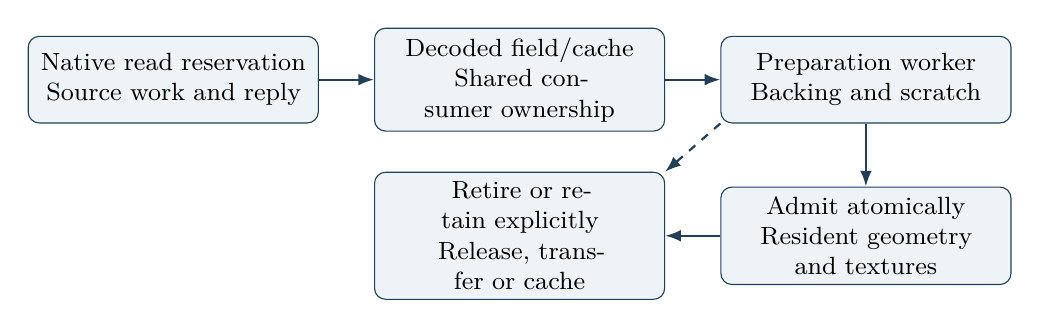
\begin{tikzpicture}[
  box/.style={draw=NimbusBlue,rounded corners,fill=NimbusLight,align=center,
    text width=3.45cm,minimum height=1.1cm,font=\small},
  flow/.style={-{Latex[length=2mm]},thick,draw=NimbusBlue}]
\node[box] (native) {Native read reservation\\Source work and reply};
\node[box,right=0.7cm of native] (field) {Decoded field/cache\\Shared consumer ownership};
\node[box,right=0.7cm of field] (worker) {Preparation worker\\Backing and scratch};
\node[box,below=0.8cm of worker] (resident) {Admit atomically\\Resident geometry\\and textures};
\node[box,left=0.7cm of resident] (retire) {Retire or retain explicitly\\Release, transfer or cache};
\draw[flow] (native) -- (field);
\draw[flow] (field) -- (worker);
\draw[flow] (worker) -- (resident);
\draw[flow] (resident) -- (retire);
\draw[flow,dashed] (worker.south west) -- (retire.north east);
\end{tikzpicture}
\caption{The I/O preference governs the first reservation, not every box.
Preparation may publish only after its resident claims are accepted. Cancelled
work and deselected layers retire their claims; reusable shared data keeps an
explicit owner.}
\end{figure}


\subsection{Admission, replacement and retirement}
A preparation task reserves the resources it expects to need. On completion,
the owner must transition construction claims to resident claims successfully
before publishing the prepared scene. If resident admission fails, the new
scene must not become visible with unaccounted backing. This commit boundary
keeps resource state and displayed state consistent.

Deselecting a volume field, replacing a preparation request or unmounting a
plot retires its inactive bricks and worker resources. Unfinished superseded
workers are stopped when their work has no remaining owner. Completed reusable
worker backing can remain warm under an explicit cache owner; that is different
from retaining every field ever selected. The corresponding error state must
also identify the current failed request rather than preserve an obsolete
failure from another field.

These rules apply to single and nested volume preparation, and to independently
required background reads. A budget increase must reach each applicable owner;
retrying only the foreground while leaving its required background failed would
leave the feature broken. Shared data stays alive while another consumer
needs it, so a drop in one pane's usage need not make every memory counter zero.

\subsection{What the resource panel can and cannot certify}
The resource panel exposes tracked ownership, reservations, resident commitments
and high-water observations. The aggregate visualization-capacity policy remains
observe-only unless a matching qualification artifact supplies the required
whole-application, GPU-residency and opaque-worker headroom evidence. Separate
native I/O limits, queue bounds, texture limits and geometry/output limits still
apply.

Observe-only does not mean unlimited memory is safe. It means that the tracked
sum is not being advertised as a universally qualified whole-application cap.
Browser subprocesses, graphics drivers, native decoder scratch and transient
runtime allocations need measurement on the actual packaged application.
An observed small-scene success is not a safe upper bound for every dataset.

\subsection{ARM64, x86-64 and memory topology}
ARM64 and x86-64 describe instruction sets. Unified and discrete memory describe
where processors access storage. Neither distinction alone predicts Studio's
performance. An ARM64 application still needs the correct runtime libraries;
an x86-64 machine can have integrated graphics; host-visible GPU memory can
still have costs unlike a tightly unified memory system.

On a discrete GPU, texture upload can create a separate device allocation and
consume interconnect bandwidth. On a unified system, CPU and GPU work still need
proper synchronization and ownership, and concurrent access can compete for the
same physical bandwidth. JavaScript arrays, worker transfers, native decoder
buffers and graphics textures do not become one shared zero-copy allocation
merely because the hardware shares memory.

Measure the viewing computer separately from a remote compute node. A remote
GPU's memory does not raise Studio's local texture capacity. Compare source
identity, field set, sampling, visible layers, worker count and graphics backend
when measuring changes. Startup, repeated-frame preparation, steady rendering,
capture and file export are separate intervals with different bottlenecks.

\section{Exporting figures and recordings}
\subsection{Choose the product to match the question}
A screenshot is a view of pixels. A numeric export preserves values and shape.
A recipe records how a view or analysis was requested. A complete reproducible
experiment also needs the source data, executable/configuration identity and
scientific inputs. These products complement one another; none silently
substitutes for all the others.

Plotly's figure controls provide image export for applicable figures. Python
numeric results support NPY and bounded CSV export; CSV is deliberately limited
because a large text expansion can consume much more memory than the array and
cannot represent arbitrary dimensionality without a declared layout. NPY
remains a supported numeric export. Use the native application for filesystem
save operations and retain meaningful filenames, units and source context.

\subsection{Exact-frame recording}
The Studio recorder offers GIF, MP4, current-frame PNG and portable HTML
viewpoints where the active renderer supports the required capture. The main
recording gate currently tracks exact rendered identities for Slice, Vector
field, Volume, Isosurface, Streamlines and Rendered supercell. The button is
disabled when the selected frame has not completed or when the active view lacks
that contract. Comparison, ensemble, investigation and research workspaces have
their own publication paths rather than borrowing an unrelated plot's receipt.

Recording selects saved-frame bounds, an output rate and a saved-frame stride.
The recorder advances to each selected frame, waits for its exact completed
identity and captures it. It does not obtain scientific correctness by sleeping
for an arbitrary fixed interval and assuming the renderer caught up. If the
source changes, the required frame is unavailable or preparation fails, the
capture operation reports the failure instead of silently repeating stale pixels.

GIF encoding is bounded: the current implementation limits encoded output to
32 MiB, 2,000 frames and a $4096\times2160$ pixel budget per frame. These are
application safeguards, not recommended scientific resolutions. Shorter ranges,
larger saved-frame strides or smaller figures can make an export fit. MP4 uses
an available FFmpeg executable, optionally selected in Settings; it is not
provided by choosing a solver GPU backend.

Portable HTML viewpoints package a finite set of captured views for another
reader to rotate among. They are not a live arbitrary-camera volume viewer or
the original three-dimensional simulation data. They are useful when the
recipient needs an accessible visual explanation without installing Studio,
provided the discretized viewpoint and source assumptions are retained.

\subsection{Capture must preserve appearance as well as time}
The frame receipt binds publication and step. A three-dimensional capture also
needs its camera, sampling and appearance settings. Lighting-only redraws
refresh the committed material description after success while preserving the
scientific endpoint. A changed shadow depth, fill tint or other material setting
must not export new pixels with a previous lighting recipe.

Legends, floors, annotations and source disclosures are part of the explanatory
image. The capture path must wait for their corresponding scene state rather
than collecting whichever DOM elements happen to exist when an asynchronous
canvas read finishes. Before sharing a figure, verify that its units, saved
time, color limits and sampling disclosure describe the claim made in its caption.

\section{Remote computation and remote workspaces}
\subsection{Run remotely, inspect locally}
The direct SSH compute workflow launches Nimbus on a named Linux connection.
The viewing computer needs OpenSSH. The remote node needs Python 3.8 or newer,
the selected Nimbus executable with the current catalog contract and an existing
writable work directory. Set up key authentication and host-key trust with the
SSH client first; Studio does not provide password or first-host-trust prompts.

Save a connection in \textbf{Settings → Compute nodes} using an SSH alias or
\texttt{user@host}, an absolute executable path and an absolute work directory.
Check connection verifies the executable and catalog. Each configuration begins
with \textbf{This computer} selected; choosing a saved node makes validation,
preflight, checkpoint inspection and launch operate on that target. Removing or
changing the selected connection cannot silently redirect a launch locally.

Optional input mappings stage local files into a job's private directory at
relative paths used by its YAML. Existing absolute mappings under the configured
remote work directory are verified against the local input rather than
overwritten. The staged YAML bytes are preserved. This prevents a successful
remote launch from quietly using a different file merely because its basename
matches an input on the viewing machine.

Confirmed completed, failed and stopped histories are received into the local
Runs directory for plotting and continuation. \emph{Receiving results} is a
separate phase, with cancellation for the transfer. A received frame is published
only after its files pass byte-count and SHA-256 checks. Transfer failure does
not erase the remote files. This workflow does not provide live streaming of
remote frames into the local viewer.

\subsection{Session ownership is deliberate}
Direct SSH runs belong to the active Studio session. Keep the viewer awake and
connected while a run is active. Quitting or losing the connection retires the
remote job through its ownership lease. This is not a detached batch-scheduler
submission workflow. An unreachable node produces an explicit error; a stop
whose outcome cannot be confirmed is reported as unconfirmed and offers retry
when connectivity returns.

A successful local Stop request is not proof that a remote process terminated.
The distinction matters when reconnecting or deciding whether another run may
use the same resources. Studio reports confirmation state rather than assume
that a network interruption implies either continued execution or completed
termination.

\subsection{A remote desktop is a separate feature}
Remote workspaces forward an existing remote browser-accessible service through
an owned SSH tunnel and open its local URL. The connection specifies host, port
and a validated URL path. Studio checks that the remote service responds; it
does not install that service or provision a remote desktop on demand.

Disconnecting this tunnel closes the viewing transport. Jobs managed within the
remote desktop remain governed by that remote environment. This differs from
the session-owned direct compute workflow above, whose launch and termination
leases are part of Studio's process contract. Choose the workflow according to
the intended owner of the remote processes, not merely because both use SSH.

\section{Diagnosing a problem without changing the science}
Start from the observed symptom and identify its owner. An I/O admission error,
a missing field, an unavailable graphics capability and a scientific runtime
rejection need different repairs. Repeatedly increasing unrelated limits can
hide the useful signal while increasing memory pressure.

\begin{longtable}{@{}p{0.29\textwidth}p{0.65\textwidth}@{}}
\toprule
Observed state & Interpretation and useful next action\\
\midrule
\endhead
Empty Runs or Open data on first launch & Expected without saved simulations.
Open a supported history or prepare a validated run. Opening the application
does not generate a demonstration storm.\\[0.6em]
No data to plot after deselection & Expected empty selection. Choose a field;
do not edit the output configuration solely because a field is off.\\[0.6em]
Field or plot unavailable & Inspect available fields, rank, units and required
geometry. A 2-D product cannot satisfy a 3-D view, and missing physical coordinates
must not be replaced by invented metre axes.\\[0.6em]
I/O request exceeds limit & Inspect the required bytes and active I/O setting.
Apply an admissible larger limit or reduce the source window. Applicable reads
retry after the changed budget is applied.\\[0.6em]
Reads waiting for memory & Other native reads own reservations. Wait, cancel
unused requests or adjust concurrency. A queue is different from a single
request that can never fit.\\[0.6em]
3-D scene is blank or faint & Check source support, finite values, opacity,
threshold, camera and graphics error state. Use a scalar slice to distinguish
absent data from a view that makes them transparent or occluded.\\[0.6em]
Blocky appearance at zoom & Inspect native spacing and sampling disclosure.
Refine a bounded view where supported. Smooth display can improve shading but
cannot create source resolution or fill missing support.\\[0.6em]
Selected time differs from image & Preparation is still running or failed.
Read the displayed-frame status; exact capture remains unavailable until the
selected publication is drawn.\\[0.6em]
Recording is disabled & The active view may lack exact-frame reporting, or its
frame is not complete. Use its supported figure/package export rather than
treat an arbitrary canvas as a verified recorder source.\\[0.6em]
MP4 encoder unavailable & Check FFmpeg discovery or its explicit path preference.
GIF and PNG have different requirements and limits.\\[0.6em]
Graphics context loss & Allow the owned scene to reconstruct; only a completed
restored render is current. Persistent failure needs inspection of scene size,
driver/webview and the reported graphics backend.\\[0.6em]
Remote termination unconfirmed & Restore connectivity and retry Stop. Do not
infer process termination from a broken network connection.\\[0.6em]
Python package import failure & Check the pinned Pyodide package path, network
availability and WebAssembly compatibility. A system-Python package installation
does not automatically populate the embedded runtime.\\
\bottomrule
\end{longtable}

A useful defect report includes application/source revision, operating system
and architecture, active graphics API, field format, domain shape, selected
plot and layers, source/frame identity, exact error text, preferences and a
small reproducible input where possible. Record whether the problem occurs on
initial load, after changing a field, during playback or during export. These
details locate the failing ownership transition more effectively than a lone
screenshot of an empty canvas.

\section{Implementation map and verification boundaries}
\subsection{Where the behavior is implemented}
The following maintained sources provide the implementation behind this guide.
The paths are relative to the repository root. They are starting points for
review, not an invitation to bypass the ordinary application path when testing a
feature.

\begin{longtable}{@{}>{\raggedright\arraybackslash}p{0.27\textwidth}>{\raggedright\arraybackslash\footnotesize}p{0.67\textwidth}@{}}
\toprule
Responsibility & Source owners\\
\midrule
\endhead
Application and plot workspace & \path{ui/src/components/studio/PlotStudio.tsx}\newline
\path{ui/src/components/runs/RunDetail.tsx}\newline
\path{ui/src/lib/plot/plotRegistry.ts}\\[0.6em]
Configuration and run admission & \path{ui/src/components/config/}\newline
\path{ui/src/lib/config/}\newline
\path{ui/src-tauri/src/commands/config_preflight.rs}\newline
\path{ui/src-tauri/src/commands/runner.rs}\\[0.6em]
Data sources and native readers & \path{ui/src/lib/dataset/}\newline
\path{ui/src/lib/run/runOutputs.ts}\newline
\path{ui/src-tauri/src/commands/outputs.rs}\newline
\path{ui/src-tauri/src/commands/netcdf_dynamic.rs}\\[0.6em]
Grid and field interpretation & \path{ui/src/lib/science/}\newline
\path{ui/src/lib/plot/renderFidelity.ts}\newline
\path{ui/src/components/plots/PlotSourceDisclosure.tsx}\\[0.6em]
2-D and 3-D views & \path{ui/src/components/plots/}\newline
\path{ui/src/components/studio/PlotCanvas.tsx}\newline
\path{ui/src/lib/vtk/}\\[0.6em]
Exact-frame and presentation state & \path{ui/src/lib/run/frameIdentity.ts}\newline
\path{ui/src/lib/run/frameReady.ts}\newline
\path{ui/src/lib/plot/panePresentationBarrier.ts}\newline
\path{ui/src/lib/vtk/coherentSceneGeneration.ts}\\[0.6em]
Context and framebuffer lifetime & \path{ui/src/lib/vtk/ownedRenderWindow.ts}\newline
\path{ui/src/lib/vtk/vtkContextRenderGuard.ts}\newline
\path{ui/src/lib/vtk/vtkTraversalGuard.ts}\\[0.6em]
Worker, cache and budget owners & \path{ui/src/lib/core/}\newline
\path{ui/src/lib/studio/studioPerformance.ts}\newline
\path{ui/src-tauri/src/commands/io_budget.rs}\newline
\path{ui/src-tauri/src/commands/worker_profile.rs}\\[0.6em]
Comparison and research & \path{ui/src/lib/comparison/}\newline
\path{ui/src/lib/research/}\newline
\path{ui/src/components/research/}\\[0.6em]
Python and external providers & \path{ui/src/lib/platform/pyodideRuntime.ts}\newline
\path{ui/src/lib/platform/pyodideWorker.ts}\newline
\path{ui/src/lib/studio/pythonWorkspace.ts}\newline
\path{ui/src/lib/derived/}\\[0.6em]
Capture and publication & \path{ui/src/components/studio/MovieRecorderDialog.tsx}\newline
\path{ui/src/lib/run/frameCapture.ts}\newline
\path{ui/src/lib/research/publication.ts}\newline
\path{ui/src/lib/studio/investigationPublication.ts}\\[0.6em]
Remote ownership & \path{ui/src-tauri/src/commands/remote_compute.rs}\newline
\path{ui/src-tauri/src/commands/remote_receive.rs}\newline
\path{ui/src-tauri/src/commands/remote_workspace.rs}\\
\bottomrule
\end{longtable}

\subsection{What bounded tests establish}
Maintained TypeScript unit checks exercise numerical display contracts,
coordinates, resource transitions, frame identities, recipe parsing and
cancellation. Browser tests exercise real mounted views, controls, rendering,
context loss, source changes and capture. Rust tests exercise native readers,
filesystem behavior, I/O admission and process ownership. Synthetic arrays and
temporary data are generated by the tests under \path{tests/ui/}; personal
simulation datasets are not application assets.

The maintained entry points include \texttt{npm run typecheck},
\texttt{npm run test:unit}, \texttt{npm run typecheck:browser},
\texttt{npm run test:browser} and the native Cargo tests. Their prerequisites
and build routes are described in \href{../ui/README.md}{the Studio source
README} and \href{BUILDING.md}{the build guide}. A test that needs a simulator,
packaged application, browser engine or external integration input must report
an unavailable prerequisite rather than convert it into a passing claim.

Chromium software rendering, WebKit, a native desktop webview and a physical GPU
are different test environments. Passing one does not automatically establish
the other three. High-density display checks and repeated mount/unmount checks
exercise additional failure modes but do not measure all driver behavior or
prove indefinite resource stability.

\subsection{Limits that remain explicit}
The application has capability-dependent paths. Missing physical coordinates
block metre-scale 3-D geometry; unavailable native provider execution remains
unavailable; exact-frame recording is limited to its implemented identity
owners; package imports depend on the embedded Python runtime; remote compute
does not provide live remote-frame streaming or detached scheduler jobs.
Aggregate whole-application capacity requires evidence beyond tracked array
sizes. These are concrete boundaries to preserve when extending the product.

Bounded repairs to cancellation, budget retry, capture metadata, resident
identity and context restoration strengthen the implemented paths. They do not
establish universal performance, all-platform readiness, completed long-running
capacity campaigns or independent scientific review. Those statuses must be
reported from the applicable evidence rather than inferred from this guide's
existence.

When expanding Studio, update the public control, reader/preparation owner,
frame and resource contracts, capture/publication metadata, tests and this
explanation together. A new visible option is complete only when the ordinary
runtime path reaches the intended behavior and its failures remain explicit.

\end{document}
